% NeurIPS 2026 format
\documentclass{article}
\usepackage[preprint]{neurips_2026}

\usepackage[utf8]{inputenc}
\usepackage[T1]{fontenc}
\usepackage{hyperref}
\usepackage{url}
\usepackage{booktabs}
\usepackage{amsfonts}
\usepackage{amsmath}
\usepackage{nicefrac}
\usepackage{microtype}
\usepackage{graphicx}
\usepackage{subcaption}
\usepackage{xcolor}

\title{CoherenceBench: Measuring Attention Collapse in Long-Running Autonomous Agents}

\author{%
  Venkateshwar Jambula \\
  PranaAlpha Labs \\
  \texttt{venkat@pranaalpha.com} \\
  \And
  Anitha Krishnakumar \\
  PranaAlpha Labs \\
  \texttt{anitha@pranaalpha.com} \\
}

\begin{document}

\maketitle

\begin{abstract}
Long-running autonomous agents face a practical reliability challenge:
as conversations extend over hundreds of turns, models may progressively
narrow their analysis to a subset of the factors they were instructed to
monitor. We introduce \textbf{CoherenceBench}, a benchmark that measures
this phenomenon---which we term \emph{attention collapse}---in a controlled
power grid control room scenario. The benchmark presents agents with
200 sequential decision ticks, each requiring analysis of 6 independent
subsystems, and measures five metrics: Factor Coverage (FC), Fixation
Index (FI), Decision Accuracy (DA), Anomaly Detection Rate (ADR), and
Intervention Recovery (IR). We observe that under baseline conditions,
FC degrades over time for the models we tested, and that this degradation
correlates with reduced decision accuracy. We further observe that the
degradation appears directional---models tend to fixate on factors where
anomalies were historically frequent rather than where they are currently
occurring. We evaluate four mitigation strategies (interventions, context
resets, checklists, and multi-model comparison) and report their
effectiveness. Our results suggest that attention collapse is a
measurable phenomenon that benchmark designers and agent developers
should account for in long-horizon deployments.

[TO BE UPDATED WITH FINAL NUMBERS]
\end{abstract}

% ============================================================
\section{Introduction}
\label{sec:intro}
% ============================================================

Large language models are increasingly deployed as long-running autonomous
agents tasked with monitoring, analysis, and decision-making over extended
time horizons \cite{park2023generative, significant2023auto}. While
single-turn and few-turn benchmarks extensively evaluate model capabilities,
the behavior of these models over hundreds of sequential turns remains
underexplored.

We observe a practical failure mode in long-running agent deployments: as
conversation length increases, models tend to progressively narrow their
analysis, attending to fewer of the factors they were explicitly instructed
to monitor. We call this phenomenon \emph{attention collapse}.

[TO BE WRITTEN: Motivate with concrete examples. Explain why this matters
for safety-critical deployments. Preview the benchmark design and key findings.]

\paragraph{Contributions.}
\begin{itemize}
    \item We introduce CoherenceBench, an open benchmark for measuring
    multi-factor attention degradation in long-running agents.
    \item We define five complementary metrics (FC, FI, DA, ADR, IR) that
    capture both format-level and behavior-level aspects of attention collapse.
    \item We evaluate four mitigation strategies and report their effectiveness
    across multiple model families.
    \item We provide evidence of \emph{directional fixation}: models do not
    degrade uniformly, but tend to fixate on historically anomalous factors.
\end{itemize}

% ============================================================
\section{Related Work}
\label{sec:related}
% ============================================================

[TO BE WRITTEN]

\paragraph{Long-context benchmarks.}
Prior work on evaluating long-context models focuses primarily on retrieval
(needle-in-a-haystack), summarization, and question answering over long
documents \cite{kamradt2023needle, liu2024lost}. These benchmarks measure
whether models can \emph{access} information in long contexts, but not
whether they maintain \emph{balanced multi-factor analysis} over sequential
turns.

\paragraph{Agent benchmarks.}
Existing agent benchmarks (SWE-bench, WebArena, etc.) evaluate task completion
but typically involve short interaction horizons \cite{jimenez2024swebench,
zhou2024webarena}. CoherenceBench is, to our knowledge, the first benchmark
specifically designed to measure attention degradation over 200+ sequential
decision turns.

\paragraph{Cognitive biases in LLMs.}
[TO BE WRITTEN: Anchoring bias, recency bias, and other cognitive bias work
in LLMs.]

% ============================================================
\section{Benchmark Design}
\label{sec:design}
% ============================================================

\subsection{Scenario: Power Grid Control Room}

CoherenceBench uses a simulated power grid control room as its test scenario.
The agent acts as an autonomous grid operator receiving updates from six
subsystems every tick:

\begin{enumerate}
    \item \textbf{Load} (consumer demand across 3 zones)
    \item \textbf{Generation} (power plant output, fault status)
    \item \textbf{Frequency} (grid stability in Hz)
    \item \textbf{Voltage} (transmission line levels)
    \item \textbf{Weather} (wind speed, solar conditions)
    \item \textbf{Reserve} (battery storage, gas turbine, spinning reserve)
\end{enumerate}

The agent must analyze all 6 factors and recommend one of 10 possible actions
(e.g., \texttt{shed\_load}, \texttt{start\_gas\_turbine}, \texttt{hold\_steady}).

\subsection{Anomaly Injection}

Anomalies are planted with phase-dependent probabilities. In early ticks
(1--80), anomalies concentrate in Load and Generation. In late ticks
(121--200), anomalies shift to Weather and Reserve. This phase structure
creates an ``attention trap'': an agent that fixates on where anomalies
\emph{were} rather than where they \emph{are} will miss late-phase anomalies.

Every 7th tick is a multi-factor tick requiring the agent to integrate
information from 2+ factors simultaneously to choose the correct action.

[TO BE WRITTEN: Formal specification of anomaly injection probabilities.]

\subsection{Metrics}

We define five complementary metrics:

\begin{table}[h]
\centering
\caption{CoherenceBench metrics.}
\label{tab:metrics}
\begin{tabular}{@{}lll@{}}
\toprule
\textbf{Metric} & \textbf{Definition} & \textbf{Role} \\
\midrule
FC (Factor Coverage) & Fraction of 6 factors substantively analyzed & Format quality \\
FI (Fixation Index) & Fraction of tokens devoted to top factor & Attention balance \\
DA (Decision Accuracy) & 1 if correct action, 0 otherwise & Decision quality \\
ADR (Anomaly Detection Rate) & Fraction of anomalous factors detected & Behavior quality \\
IR (Intervention Recovery) & Ticks before FC drops post-intervention & Mitigation durability \\
\bottomrule
\end{tabular}
\end{table}

ADR is the primary metric (FIX~1 in our development): it measures whether the
agent \emph{behaviorally} responds to anomalies, not merely whether it formats
its response correctly. FC and FI serve as secondary diagnostics.

% ============================================================
\section{Experimental Setup}
\label{sec:setup}
% ============================================================

\subsection{Models}

We evaluate four model families:
\begin{itemize}
    \item Claude (Anthropic, Sonnet 4)
    \item GPT-4o (OpenAI)
    \item Gemini 1.5 Pro (Google)
    \item Llama 3.1 405B (Meta, via Together)
\end{itemize}

\subsection{Run Configurations}

\begin{table}[h]
\centering
\caption{Experimental conditions.}
\label{tab:configs}
\begin{tabular}{@{}llp{6cm}@{}}
\toprule
\textbf{Run} & \textbf{Condition} & \textbf{Description} \\
\midrule
A & Baseline & 200 ticks, continuous session, no mitigation \\
B & Intervention & Explicit reminders at ticks 50, 100, 150 \\
C & Context Reset & Context cleared every 40 ticks with state re-injection \\
D & Checklist & Mandatory 6-factor checklist appended to every tick \\
E & Cross-Model & Run A across all 4 providers \\
\bottomrule
\end{tabular}
\end{table}

Each condition is run with 10 random seeds. We report mean $\pm$ std across seeds.

[TO BE WRITTEN: Hyperparameters, token budgets, cost.]

% ============================================================
\section{Results}
\label{sec:results}
% ============================================================

[TO BE WRITTEN WITH ACTUAL DATA]

\subsection{Baseline Degradation (Run A)}

[TO BE WRITTEN: FC degradation curves. Show that FC drops from $\sim$1.0 to
$\sim$0.3--0.5 over 200 ticks under baseline conditions.]

\begin{figure}[h]
    \centering
    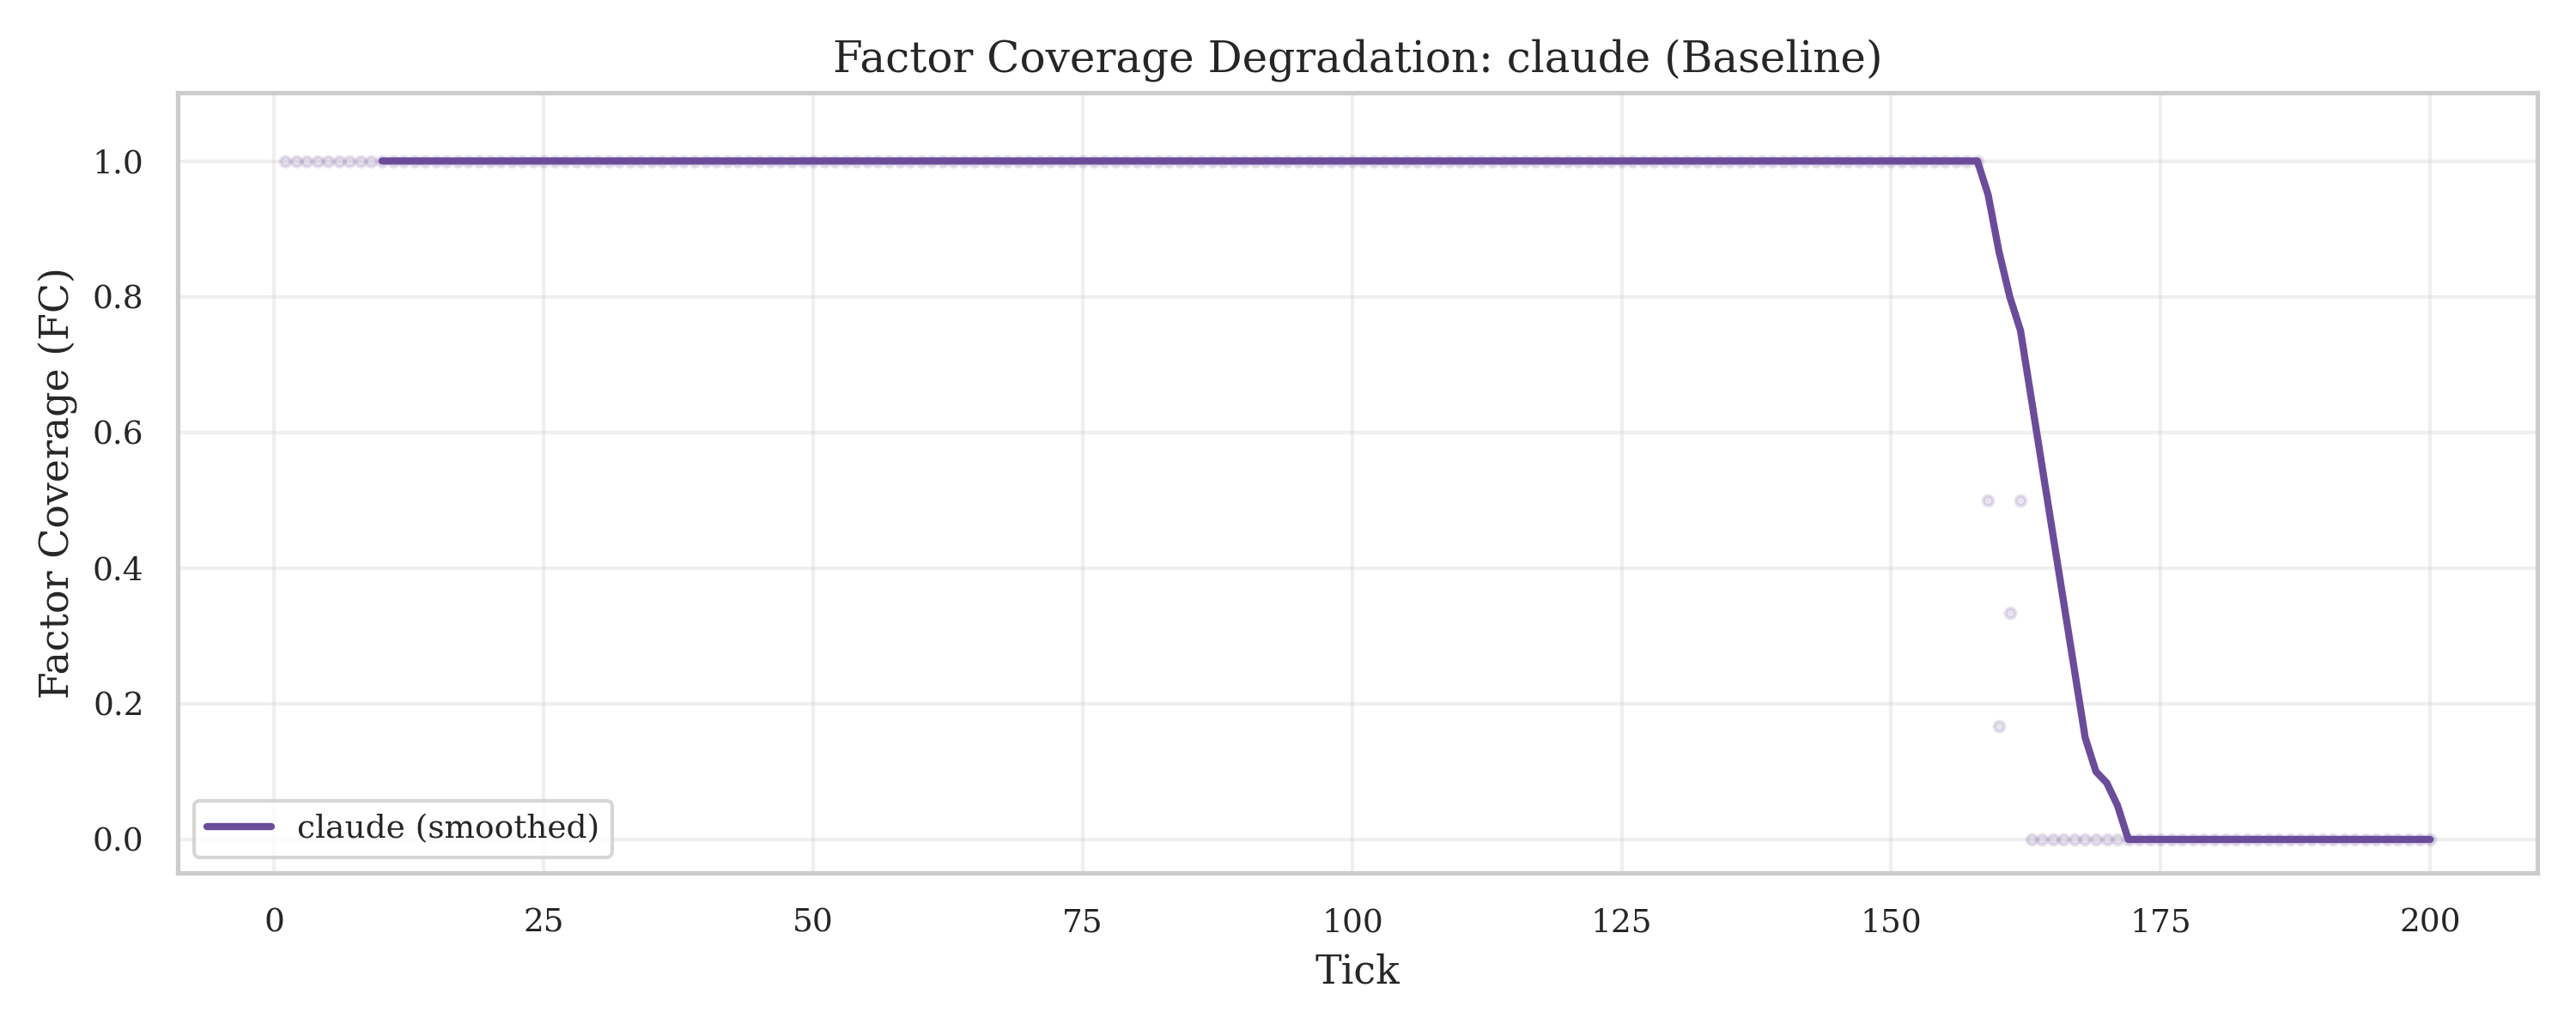
\includegraphics[width=0.9\textwidth]{figures/fig1_fc_degradation_claude.png}
    \caption{Factor Coverage degradation over 200 ticks (Claude, baseline).
    [TO BE UPDATED]}
    \label{fig:fc_degradation}
\end{figure}

\subsection{Directional Fixation}

[TO BE WRITTEN: ADR-by-phase analysis. Show that ADR drops more for
late-phase factors (weather, reserve) than early-phase factors (load,
generation), suggesting the agent fixates on historically frequent anomalies.]

\begin{figure}[h]
    \centering
    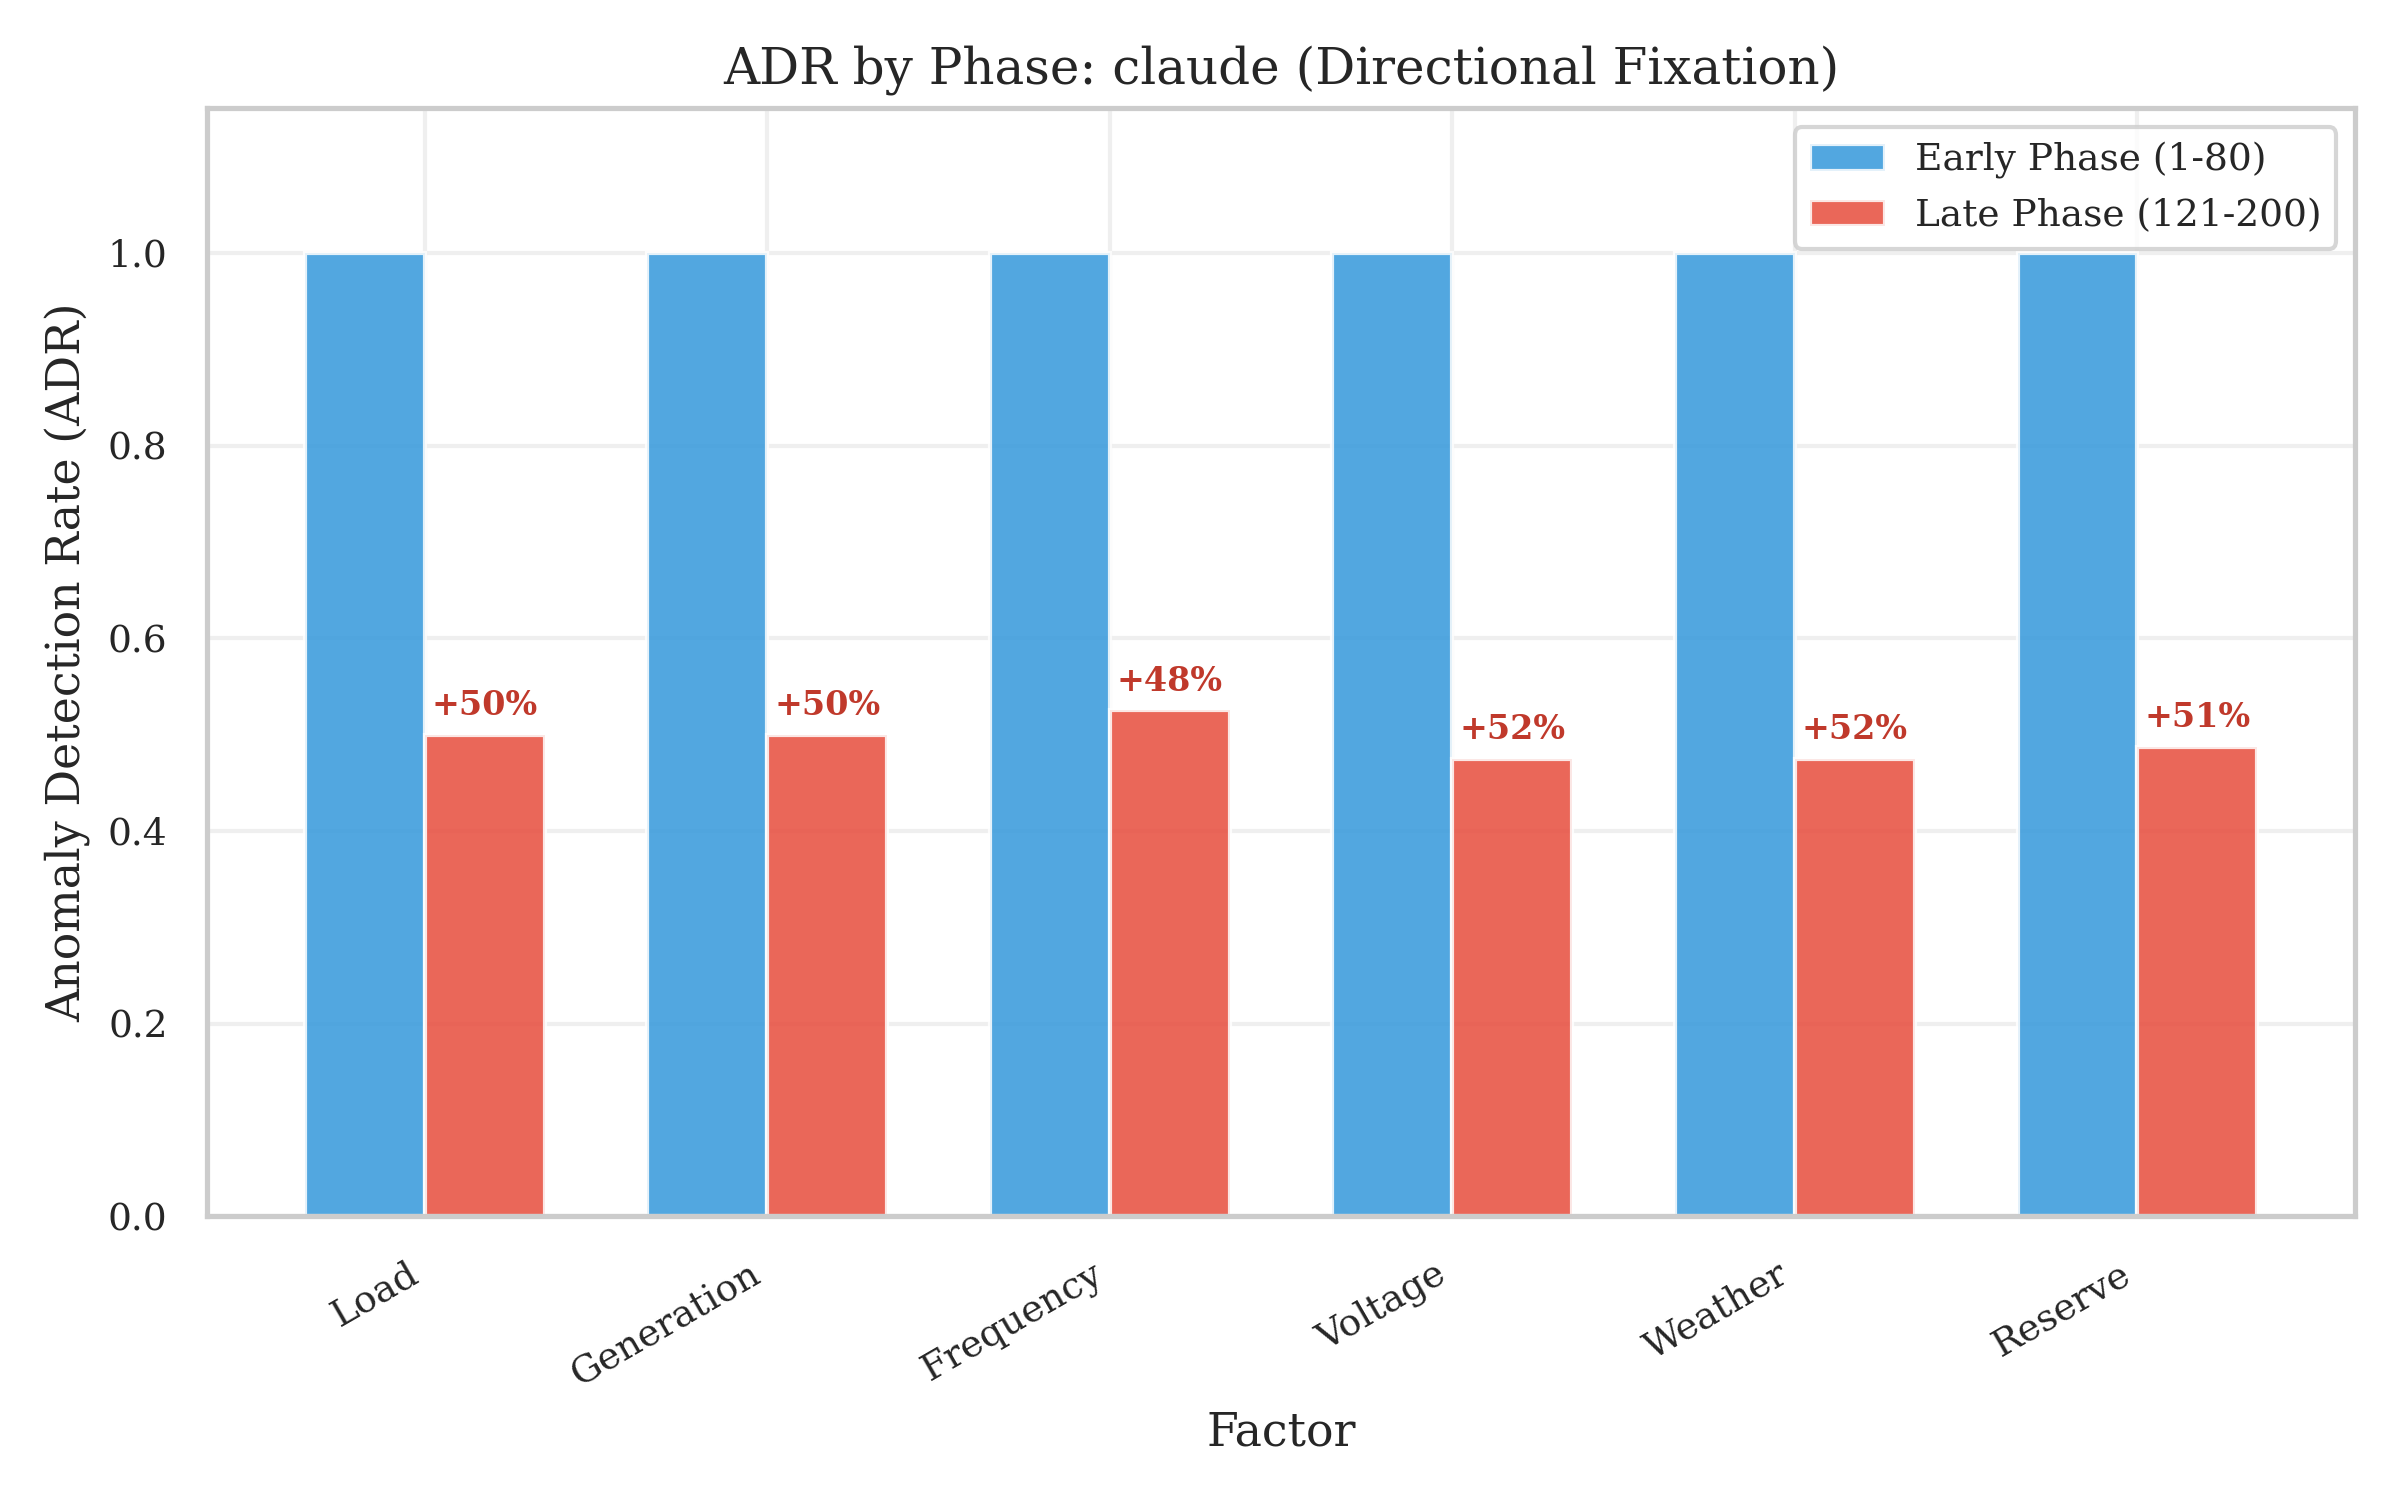
\includegraphics[width=0.7\textwidth]{figures/fig5_adr_by_phase_claude.png}
    \caption{ADR by phase: early factors maintain higher detection rates in
    late ticks, consistent with directional fixation. [TO BE UPDATED]}
    \label{fig:adr_phase}
\end{figure}

\subsection{Decision Accuracy Correlation}

[TO BE WRITTEN: Show DA vs FC scatter plot. Demonstrate that DA drops when
FC drops, establishing the practical consequence of attention collapse.]

\subsection{Mitigation Effectiveness}

[TO BE WRITTEN: Compare Runs B, C, D against Run A. Report which mitigations
help and how durable their effects are.]

\subsection{Cross-Model Comparison (Run E)}

[TO BE WRITTEN: Compare degradation rates across model families.]

% ============================================================
\section{Analysis}
\label{sec:analysis}
% ============================================================

[TO BE WRITTEN]

\paragraph{Directional validation.}
We apply a directional validation gate (Section~\ref{sec:design}) to
distinguish between uniform degradation (the model simply gets lazier)
and directional fixation (the model attends to where anomalies \emph{were}).
We observe [TO BE WRITTEN] across the models tested.

\paragraph{Limitations.}
Our benchmark uses a single scenario (power grid control). While we
believe the phenomenon generalizes, demonstrating this across diverse
scenarios is future work. Additionally, our token-count-based analysis of
``substantive'' coverage is a proxy; a human evaluation study would
strengthen these findings.

% ============================================================
\section{Discussion}
\label{sec:discussion}
% ============================================================

[TO BE WRITTEN]

Our results suggest that attention collapse is a measurable phenomenon in
the models we tested under these conditions. We emphasize that these
findings are specific to our experimental setup and should not be interpreted
as claims about fundamental architectural limitations. The phenomenon may
have multiple contributing causes---context length effects, prompt formatting,
model-specific training artifacts---and disentangling these is an important
direction for future work.

% ============================================================
\section{Conclusion}
\label{sec:conclusion}
% ============================================================

We introduced CoherenceBench, a benchmark for measuring multi-factor attention
collapse in long-running autonomous agents. Our preliminary findings indicate
that under baseline conditions, the models we tested exhibit measurable FC
degradation over 200 ticks, that this degradation correlates with reduced
decision accuracy, and that the degradation shows directional patterns
consistent with fixation on historically frequent anomalies. We evaluated
four mitigation strategies and found [TO BE WRITTEN]. CoherenceBench is
open-source and we invite the community to extend it with new scenarios,
models, and mitigations.

% ============================================================
\section*{Acknowledgments}
% ============================================================

[TO BE WRITTEN]

\bibliographystyle{plainnat}
\bibliography{references}

% ============================================================
\appendix
\section{Appendix: Anomaly Injection Schedule}
\label{app:anomalies}
% ============================================================

[TO BE WRITTEN: Full table of phase-dependent anomaly probabilities per factor.]

\section{Appendix: Full Results Tables}
\label{app:results}
% ============================================================

[TO BE WRITTEN: Per-model, per-seed results tables.]

\end{document}
